\documentclass[12pt]{article}
\usepackage[margin=1in]{geometry}
\usepackage{mathrsfs}
\usepackage{amsmath}
\usepackage[font={small,it}]{caption}
\usepackage{subcaption}
%\usepackage{pxfonts}
\usepackage[sc]{mathpazo}
\usepackage{authblk}
\usepackage{lineno}
\usepackage{graphicx}
\graphicspath{{/home/conor/Dropbox/PhD/PhD_NMBU/PaperIV/GooldNewberry2020-lba/paper/figures/}}
\linespread{1.15}
\usepackage{hyperref}
\hypersetup{
  colorlinks=false
}

\usepackage[
  backend=biber,
  citestyle = authoryear,
  bibstyle = authoryear,
  giveninits=true,
  maxcitenames=2,
  uniquelist=false,
  uniquename=false,
  useprefix=true
  ]{biblatex}
\usepackage[utf8]{inputenc}
\usepackage[T1]{fontenc}
\addbibresource{~/Dropbox/PhD/PhD_NMBU/PaperIV/GooldNewberry2020-lba/paper/GooldNewberry2020-refs.bib}

\title{Longitudinal behavioural assessment of shelter dogs predicts behaviour post-adoption}
\author[1,2]{Conor Goold}
\author[2]{Ruth C. Newberry}
\affil[1]{\small{Faculty of Biological Sciences, University of Leeds, UK, LS2 9JT}}
\affil[2]{\small{Department of Animal and Aquacultural Sciences, Norwegian University of Life Sciences, \r{A}s, Norway}}
\date{}
\begin{document}
\linenumbers
\modulolinenumbers[5]

\maketitle

\begin{abstract}
  \small
  Predicting the behaviour of shelter dogs after adoption is an important, but difficult, endeavour. Despite three decades of research on behaviour assessments in shelters, evidence supporting their use is mixed. In part, this is due to the use of behaviour test batteries conducted soon after the dog arrives to a shelter, which have questionable test validity and high chances of producing false positives. This study provides the first analysis of the ability for a longitudinal, observational behaviour assessment to predict behaviour post-adoption. We analyse shelter behavioural observations ($> 60,000$ records in total) and post-adoption behavioural reports (using telephone surveys) across eight contexts from 241 dogs. A novel joint hierarchical Bayesian mixture model is used to i) compare shelter and post-adoption behaviour, ii) model the impact and predictors of missing data, and iii) understand potential measurement error in shelter and post-adoption behavioural records. Dog behaviour at the shelter correlated positively with behaviour post-adoption within contexts (0.38; 95\% highest density interval: [0.20, 0.57]). [...]
\end{abstract}
\newpage
\tableofcontents

\section{Introduction}
Accurately predicting the future behaviour of domestic dogs (\textit{Canis familiaris}) is a priority for professional organisations, dog breeders, and dog owners alike. Animal shelters have the difficult task of assessing how dogs will behave in a variety of circumstances from limited behavioural information, and making decisions about the suitability of those dogs for placement into new homes. To do so, animal shelters frequently employ standardised behaviour tests that evaluate specific behavioural or \textit{personality} traits through reconstructions of situations relevant to life outside the shelter environment (\cite{vanderborg1991}; \cite{marston2003}; \cite{mornement2010}; \cite{taylor2006}; \cite{rayment2015}). For example, to assess a dog's level of aggressiveness around food (i.e. food guarding), shelter staff may present a dog with a bowl of food and record the dog's response to a plastic hand approaching, touching or trying to remove the food bowl (\cite{mohangibbons2012}; \cite{mohangibbons2018}; \cite{marder2013}). Standardised tests are usually conducted once, soon after arrival at the shelter, yielding an overall score used to help determine the dog's suitability for adoption.

Despite three decades of research on the development, implementation and predictive validity of shelter dog behavioural assessments, the evidence supporting their use is mixed. The reliability and validity of many behavioural assessments used by shelters have not been ascertained (\cite{taylor2006}; \cite{mornement2009}; \cite{mornement2010}; \cite{mornement2014}). The feasibility of carrying out behavioural assessments with high reliability and standardisation in the time-constrained shelter environment has also been questioned, with assessments often taking at least an hour per dog (\cite{vanderborg1991}; \cite{mornement2009}; although see \textcite{poulsen2010} for a shorter evaluation). In the last ten years, criticisms have been levelled against the ability for behavioural assessments to predict dog behaviour after adoption with reasonable accuracy. A high number of false positives have been recorded for food guarding behaviour (i.e. displaying food aggression during shelter evaluations but not in the new home; see \cite{mohangibbons2012}; \cite{marder2013}) and has led to calls for abandoning standardised food tests after return rates to shelters did not increase when the tests had been terminated (\cite{mohangibbons2018}). Other types of aggressive and non-aggressive behaviours might be similarly difficult to predict post-adoption (\cite{christensen2007}; \cite{mornement2015}; although see \textcite{bollen2008}).

The reasons why dog behaviour is difficult to predict post-adoption are varied, and ways to improve predictions are not entirely clear. Widespread advice to improve the reliability and validity of shelter dog assessments are hampered by a lack of clarity of what those terms mean (\cite{patronek2019}; \cite{rayment2015}), which is also a problem in the wider scientific community (e.g. see \cite{borsboom2004}; \cite{borsboom2009}; \cite{maul2016}). \textcite{patbrad2016} demonstrate that even with high sensitivity and specificity, the probability of a dog showing aggression in the new home after a positive test in the shelter is unlikely to be higher than 50\%, and is probably closer to $\sim$ 30\% (see also \cite{patronek2019}). Tests that have been reported to predict behaviour successfully post-adoption (e.g. \cite{valsecchi2011}; \cite{poulsen2010}; \cite{bollen2008}) support their claims using statistical significance of linear associations (e.g. significant correlations or regression coefficients) between shelter and post-adoption behaviour (i.e. predictive `validity'; \cite{patronek2019}). In constrast, studies arguing against the efficacy of behavioural tests do so with (arguably more relevant) evidence of low predictive `ability', i.e. estimates of true/false positive and negative rates (\cite{patronek2019}). As an alternative, a number of authors and organisations emphasise the collection of daily behavioural observations from dogs in shelters, in addition to other information (e.g. foster reports, pre-surrending interviews), to formulate a holistic profile of each dog's behaviour and welfare needs used to inform adoption (\cite{patronek2019}; \cite{ASPCA2018}; \cite{rayment2015}; \cite{mornement2015}). However, research is still scarce on how best to implement this approach and summarise the swathes of information observational methods generate on each dog to be of practical use for shelters.

In previous studies, we have reported on the behaviour of dogs in shelters from a longitudinal and observational assessment methodology implemented in one UK shelter (\cite{goold2017aggressiveness}; \cite{goold2017modelling}). The assessment relies on the sponataneous collection of behavioural observations from everyday occurrences (e.g. walking past the dog's kennel, putting a food bowl into the kennel, clipping on the lead or touching the collar) to cumulatively determine how best to maintain the dog's welfare and place into a new home. \textcite{goold2017modelling} used the framework of behavioural reaction norms (\cite{dingemanse2010}; \cite{cleasby2015}) to partition individual variation in over 3,000 dogs' behaviours ($\sim$ 20,000 behavioural reports in total) around unknown people into personality (i.e. average behaviour), plasticity (i.e. behavioural change over time at the shelter) and predictability (i.e. residual variance). Accounting for all three components improved the out-of-sample predictive accuracy of the statistical models. In addition, we found large uncertainty in the estimates of personality, plasticity and predictability, in part due to the varying number of observations present for each dog.

The goal of the present study was to assess the correspondance between behaviour shown at the shelter, collected using the longitudinal observation methodology, and the behaviour reported during telephone interviews post-adoption. To do so, we present a novel application of joint Bayesian hierarchical modelling that accounts for: i) individual variation in both personality and plasticity (due to only two post-adoption interviews, predictability was not estimated) across shelter and post-adoption time periods; ii) missing data and their potential correlates; iii) measurement error in the behavioural reports. We report on predictive validity by estimating correlations between personality and plasticity between shelter and post-adoption time periods, and predictive ability by using posterior predictions from our model to calculate the number of dogs that changed their behaviour between shelter and post-adoption time periods in meaningful ways.

\section{Materials \& Methods}

\subsection{Subjects}
Behavioural data were gathered retrospectively from new owners on 265 dogs adopted from Battersea Dogs and Cats Home, United Kingdom between May 2016 and May 2017. Details of the shelter environment can be found in \textcite{goold2017aggressiveness} and \textcite{goold2017modelling}. Of the 265 dogs, only 241 dogs could be matched with behavioural and demograhpic data from the shelter's database. Demographic information about these dogs is presented in Table \ref{table_demoshelter}. Demographic information of the new owners was collected but not analysed here due to inconsistencies in the responses.

\begin{table}
  \centering
  \begin{tabular}{ll}
  \textbf{Demographic variable} & \textbf{Mean (SD)/$\boldsymbol{n}$}\\ \hline
  Number of total observations per dog & 140.7 (224.3) \\
  Days spent at the shelter & 32.1 (41.4)\\
  Estimated age at departure (years) & 3.6 (2.8)\\
  Weight (kg; last recorded at shelter) & 16.5 (9.6)\\
  Source: gift/stray/return & 164/51/26\\
  Rehoming centre: London/Old Windsor/Brands Hatch & 71/93/77\\
  Sex: female/males & 102/139\\
  Neutered: before arrival/at shelter/not/missing & 84/145/11/1 \\ \hline
  \end{tabular}
  \caption{Dog demographic variables collected at the shelter.}
  \label{table_demoshelter}
\end{table}

\subsection{Data collection}

\subsubsection{Shelter behaviour}
As previously described by \textcite{goold2017aggressiveness} and \textcite{goold2017modelling}, shelter employees observed dogs in a variety of naturally-occurring contexts (Table \ref{table_contexts}) and recorded each dog's behaviour using a context-specific list of mutually-exclusive behavioural codes. The contexts analysed here were eight core ‘on-site' contexts. The \textit{Interactions with dogs} context was a combination of the original \textit{Interactions with female} and \textit{male dogs} contexts, respectively, because the post-adoption data did not distinguish between interactions with male and female dogs (as adopters may not have been fully aware of the sex of other dogs that their dog met). Observations were made as often as possible given the frequency the situation occurred and the time constraints on entering data for shelter staff. However, we consider any day the dog did not receive an observation in a context as a missing observation so that patterns of missingness could be modelled (see Table \ref{table_contexts} for amount of missing daily observations). In total, there were $61,952$ (missing and complete) observations in the shelter dataset.

There were between ten and sixteen possible behavioural codes depending on the context, arranged on a scale of perceived ease of adoption or desirability to adopters (see Supplementary Materials for the full list of behavioural codes). The behavioural codes were further categorised by the shelter into green, amber and red categories: green codes indicated that the dog's behaviour was suitable for immediate adoption and/or would be easy for all owners to manage once adopted (e.g. the dog was friendly or excited when meeting new people), amber codes indicated that some training or management might be needed to manage or improve behaviour (e.g. the dog was nervous when meeting new people and slow to meet with them), and red codes that the dog needed an individualised training program and improvement in behaviour to facilitate adoption or would be the most difficult for adopters to manage (e.g. the dog showed aggression when meeting unfamiliar people). A dog's suitability for adoption was decided based on behaviour across all contexts and days after arrival. Dogs were not adopted to the public if they were considered to pose a serious and highly probable risk towards people or other dogs.

\begin{table}[t!]
  \centering
  \small
  \begin{tabular}{p{4cm}p{6cm}p{3cm}p{3cm}}
    \textbf{Context} & \textbf{Description} & \textbf{Median (IQR)} & \textbf{\% Missing (SD)}\\ \hline
    Handling (HND) & \footnotesize{Informal handling by people (e.g. stroking non-sensitive areas, touching or holding the collar, fitting a harness or lead).} & 13 (14) & 40 (20) \\
    In kennel (KNL) & \footnotesize{Inside the kennel} & 14 (14) & 37 (21) \\
    Outside the kennel (OKNL) & \footnotesize{Outside the kennel} & 13 (14) & 42 (19)\\
    Interactions with familiar people (FPL) & \footnotesize{Interacts with familiar people (interacted with at least once before) outside the kennel who approach, make eye contact, speak to or attempt to make physical contact with the dog.} & 13 (14) & 44 (18)\\
    Interactions with unfamiliar people (UFPL) & \footnotesize{Interacts with familiar people (never interacted with before) outside the kennel who approach, make eye contact, speak to or attempt to make physical contact with the dog.} & 6 (5) & 75 (15)\\
    Eating food (FOOD) & \footnotesize{Eating food from a container, toy or while being hand-fed} & 14 (13) & 39 (20)\\
    Interactions with toys (TOYS) & \footnotesize{Interacting with dog toys} & 8 (13) & 58 (25) \\
    Interactions with dogs (DOGS) & \footnotesize{Meeting dogs outside the kennel during structured interactions and/or sponataneous meetings} & 5 (4) & 76 (12) \\
    \hline
  \end{tabular}
  \caption{Observational contexts at the shelter with corresponding median and interquartile range (IQR; due to skewness) of the number of records per dog, and average percentage (standard deviation) of missing daily records per dog.}
  \label{table_contexts}
\end{table}

The behavioural scores were analysed using the green, amber and red ordinal scale, rather than using the individual behavioural codes of each ethogram. This was chosen: i) to place the behaviour records across contexts on a comparable scale, allowing all the data to be analysed within the same statistical model; ii) to capture the main variation in the data given that some individual codes were seldom used; iii) because previous analysis indicated higher consensus among shelter staff when rating behaviour using the green, amber and red codes than the individual codes (see \cite{goold2017modelling}); and iv) it was more practically relevant because the shelter was interested to find out if their assessments at the shelter differed greatly from a dog's behaviour post-adoption (i.e. there was a change from green to red codes), but not necessarily if there was a change between codes within the same colour category. When more than one record was made of the same dog in the same context on the same day, the most `severe' code assigned was retained for analysis.

\subsubsection{Post-adoption behaviour}
On the point of adoption, adopters were asked to participate in a study evaluating the predictive accuracy of the shelter's behavioural assessment and were given full details of the procedure (consent form provided in the Supplementary Materials). Each consenting adopter received two phone calls from a canine behaviourist at the shelter who surveyed them about their dog's behaviour using a standardised set of questions (provided in the Supplementary Materials). The majority of phone calls were made by one behaviourist although no records were kept on which behaviourist made the calls. The study planned to record behaviour using telephone interviews at approximately 2-3 weeks and 5-6 weeks after adoption, but the real days after adoption were more variable. The average number of days after adoption for the first phone call was 19.8 (sd = 4.9; range = 7 to 51), and 32.7 days (sd = 11.1; range = 14 to 72) for the second, with an average of 20.7 (sd = 5.6; range = 4 to 42) days between first and second surveys for those dogs with two completed surveys. Only 150 dogs (62\%) had two completed surveys.

The first questions gathered information about the adopters' dog ownership experience and the post-adoption environment. The remaining questions (Table \ref{table_postadoptq}) enquired about how the dog reacted in situations comparable to the eight behavioural observation contexts in the shelter assessment (Table \ref{table_contexts}). The questions were used as a guide during the post-adoption interviews, with the behaviourists providing more detailed descriptions as needed. One additional context (‘\textit{How has the dog behaved when with any other resource?}’) had too few records in either the post-adoption reports or at the shelter to be included in the analysis. The \textit{In kennel} and \textit{Out of kennel} contexts at the shelter were transformed to \textit{In house} and \textit{Out of house}. The questions were open-ended, with the behaviourist encouraging adopters to describe the dog's behaviour in each situation rather than label the behaviour. Subsequently, the behaviourist chose the behavioural code for each context that best described the behaviour. Adopters were allowed to respond `No opinion'. Phone calls were not recorded, precluding assessment of the reliability of behaviour coding during phone calls. Data were handled anonymously by the authors, who received only the dogs' identification numbers to enable matching of the post-adoption reports with the shelter records.

\begin{table}
  \centering
  \begin{tabular}{p{6cm}p{6cm}p{4cm}}
    \textbf{Context (abbreviation)} & \textbf{Survey question} & \textbf{$\boldsymbol{n}$ (\%) 2 surveys}\\ \hline
    Handling (HND) & \footnotesize{How has the dog behaved whilst being handled or restrained (informal)?} & 149 (61.8)\\
    In house (HOUSE) & \footnotesize{How has the dog behaved in the house?} & 149 (61.8)\\
    Out of house (OSTD) & \footnotesize{How has the dog behaved outside on walks?} & 147 (61.0)\\
    Interactions with familiar people (FPL) & \footnotesize{How has the dog behaved when meeting familiar people?} & 144 (59.8)\\
    Interactions with unfamiliar people (UFPL) & \footnotesize{How has the dog behaved when meeting unfamiliar people} & 149 (61.8)\\
    Eating food (FOOD) & \footnotesize{How has the dog behaved with their food?} & 150 (62.2)\\
    Interactions with toys (TOYS) & \footnotesize{How has the dog behaved with toys?} & 149 (61.8)\\
    Interactions with dogs (DOGS) & \footnotesize{How has the dog behaved when meeting another dog for the first time?} & 144 (59.8)\\
    \hline
  \end{tabular}
  \caption{Post-adoption survey behaviour questions and response rates (number and percentage of owners responding to the question over two surveys).}
  \label{table_postadoptq}
\end{table}

\subsection{Statistical analysis}

\subsubsection{Theoretical approach}\label{sec_theoretical_approach}
The red-green-amber codes from shelter and post-adoption time points were analysed using a joint or `shared parameter' (e.g. see \cite{vonesh2006}; \cite{tseng2016}) Bayesian hierarchical model, which accounted for two data complexities. First, we treated the missing data present in the shelter records (Table \ref{table_contexts}) and post-adoption surveys (Table \ref{table_postadoptq}) as non-ignorable (i.e. not random) because they likely depended on other variables. For example, the number of people unfamiliar to a dog decreases with time spent at the shelter or time after adoption, leading to potentially more missing records with days after arrival in the \textit{Interactions with unfamiliar people} context. A dog’s overall behaviour could also impact missing values. For example, dogs who have more green codes overall and do not change their behaviour may not receive as many records due to a lack of priority over dogs who show more worrying behaviour. The participation or attrition rate of adopters in the telephone surveys may also have depended on their dog’s behaviour post-adoption.

A second complexity was the high proportion ($\sim$ 90\%) of green codes, which was found in previous analysis of the same shelter assessment (\cite{goold2017modelling}). We hypothesised here that some proportion of the green codes could have been recorded due to other processes, such as staff members not observing the dog’s behaviour directly, or forgetting how a dog behaved, but inputting a green code anyway. Adopters may have also described their dog’s behaviour in terms consistent with green codes (i.e. not reporting any problems) during phone calls when the dog’s behaviour might be more consistent with amber or red code behaviour. Thus, if not missing, some green codes were potentially ‘inflated’, leading to a greater probability mass for green codes beyond that explained by the data generating processes of the behavioural scale alone. Similar assumptions are applied to count data with a high number of zero values (zero inflation; \cite{lambert1992}), and have also been used to understand a high probability mass for ‘I don’t know’ responses (\cite{kelley2008}) and ‘face-saving’ or ‘Neither agree nor disagree’ responses (\cite{bagozzi2012}) on ordinal survey scales.

To account for the above complexities, we specified a custom mixture model for the probability of different codes ($c = {\text{missing}, \text{green}, \text{amber}, \text{red}} = {0, 1, 2, 3}$) for case $i$ (either the day at the shelter or the day after adoption), dog $j$ and context $k$:

\begin{equation}
  p(y_{ijk}^{c}) =
  \begin{cases}
      \psi_{ijk} & \text{if } y_{ijk} = 0 \\
      (1-\psi_{ijk})\big[\kappa + (1-\kappa)\pi_{ijk}^c\big]
      & \text{if } y_{ijk} = 1 \\
      (1-\psi_{ijk})(1-\kappa)\pi_{ijk}^c
      & \text{if } 1 < y_{ijk} \leq 3
  \end{cases}
  \label{eq_mixture}
\end{equation}

The parameter $\psi_{ijk}$ is a ‘hurdle’ probability of missing data for each dog and context (see \cite{kubinec2019} for a similar approach to handling missing data), which is modelled as a Bernoulli trial from the data:

\begin{equation}
  y_{ijk}^{c} \big|_{c=0} \sim \text{Bernoulli}(\psi_{ijk})
  \label{eq_missing}
\end{equation}

The complement, $1 - \psi_{ijk}$, is the probability of either a staff member choosing to input an observation in the shelter or an adopter participating in the telephone survey, respectively. The $\kappa$ parameter is a mixing term that describes the probability of a green code being drawn from the inflation component. Consequently,  $1 - \kappa$ is the probability of a code being non-inflated. A non-missing and non-inflated code of cateogory $c$ (and for a specific case, dog and context) occurs with probability $\pi_{ijk}^c$, which is defined using a cumulative ordinal probit model:

\begin{equation}
  y_{ijk}^{c} \big|_{c=\{1,2,3\}, 1 - \kappa} \sim \text{Categorical}(\pi_{ijk}^c)
  \label{eq_cat}
\end{equation}

\begin{equation}
  \pi_{ijk}^c = \Phi \Big( \frac{\theta_{c} - \mu_{ijk}}{\sigma} \Big) - \Phi \Big( \frac{\theta_{c-1} - \mu_{ijk}}{\sigma} \Big)
  \label{eq_ordprob}
\end{equation}

Equation \ref{eq_cat} describes the non-missing and non-inflated code as categorically distributed with probability $\pi_{ijk}^c$, which is defined in equation \ref{eq_ordprob} as the cumulative area under a latent standard normal distribution (where $\Phi$ is the standard normal cumulative distribution function) between threshold parameters $\theta_{c}$ and $\theta_{c-1}$ ($\boldsymbol{\theta} = {\theta_{0}, \theta_{1}, \theta_{2}, \theta_{3}}$). The probability of the first and last threshold parameters (i.e. $\Phi({\theta_{0}})$, $\Phi({\theta_{3}})$) were set to 0 and 1, respectively. To estimate the mean ($\mu_{ijk}$) and standard deviation ($\sigma$) on the scale of the ordinal data, we fixed $\theta_{1} = 1.5$ and $\theta_{2} = 2.5$ (see \cite{kruschke2014}).

\subsubsection{Shelter and post-adoption sub-models}
The data from the shelter and post-adoption time periods were each analysed by the model described above, which we describe as two distinct `sub-models'. For the shelter sub-model, we included days after arrival as an observation-level predictor and the variables from Table \ref{table_demoshelter}, save the total number of observations (which was nearly perfectly collinear with length of stay) and rehoming centre (which was not of interest), as dog-level predictors on both the probability of missing data ($\psi_{ijk}$ in equation \ref{eq_missing} using a logit link function) and the predicted mean of the latent behavioural scale ($\mu_{ijk}$ in equation \ref{eq_ordprob} using the identity link function). For the post-adoption sub-model, we predicted the probability of missing data and the latent behavioural scale scores using days after adoption as an observation-level predictor and the same shelter demographic variables as in the shelter sub-model as retrospective dog-level predictors, as well as the total number of surveys the dog had as an additional dog-level predictor. Sum-to-zero coding was used for categorical predictors. Dog-level metric predictors were mean-centered and standardised by 1 standard deviation. Days after adoption was centered around the average of each dog's mean number of days after adoption (26.3 days) and scaled by the standard deviation ($\sim$ 6 days). days after arrival was centered around the average length of stay at the shelter (32.1; \ref{table_demoshelter}) and scaled by 1 standard deviation. One dog had missing neuter status data, two dogs were missing weight data and two dogs were missing age at departure data. Due to the small amount, we imputed the missing neuter status data point with the most frequent category (neutered on site; Table \ref{table_demoshelter}), and mean imputed the missing weight and age data points.

Each sub-model included dog-, context-, and dog $\times$ context-varying intercept and slope (for the days after arrival or days after adoption, respectively) parameters. The joint aspect of our model derives from correlations between these parameters across the shelter and post-adoption sub-models. For the ordinal probit regressions (equation \ref{eq_ordprob}), we included random intercepts and slope terms for dogs, contexts and the interaction between dogs and contexts ($1,928$ unique dog $\times$ contexts combinations). Dog- and context-varying effects capture additive variation due to dogs and contexts, respectively, while the dog $\times$ context interaction describes the non-additive, unique variation attributed to specific dogs in specific contexts. For the missing data binary-logistic regressions, we included only random intercepts. For each random effect term (dogs, contexts, and dogs $\times$ contexts), this led to a 6 x 6 covariance matrix capturing the relationship between random intercepts and slopes for the shelter and post-adoption behaviours.

\subsubsection{Estimation \& inference}
All data cleaning and post-processing was conducted in R version 3.6.1 (\cite{rcoreteam2019}). We fit our model using Bayesian estimation in the Stan programming language (\cite{stan2018}) using the terminal interface CmdStan version 2.23.0 (\cite{cmdstan2018}). Stan employs Hamiltonion Monte Carlo, a type of Markov chain Monte Carlo (MCMC) sampling algorithm, to sample from the posterior distribution. After ensuring adequate mixing of multile chains from the model ran on smaller sub-sets of the data, we took 10,000 iterations from the posterior distribution using 2 MCMC chains (1000 warmup and 5000 sampling). We summarise parameters by their means and 95\% highest density intervals (HDIs). For the ordinal data, we make predictions using both the latent metric scale and the corresponding posterior probabilities of each ordinal category. When evaluating population-level parameters, we highlight discrepancies, where appropriate, between the estimates for average dogs and contexts, and estimates that incorporate uncertainty due to variation across dogs and contexts. The former represent estimates made at the mean of the random effects, while the latter are made by computing predictions marginal of the random-effect distributions and are particularly important for making accurate future predictions in hierarchical models (e.g. \cite{inthout2016}; \cite{wang2019}).

\subsection{Ethical statement}
Approval for the processing of personal data was gained from the Norwegian Social Science Data Services (approval number 47080). Names and addresses of the participating new owners and their dogs were anonymised before data were passed to the authors.

\subsection{Data \& code accessibility}
We provide complete mathematical details of the above model, supplementary files, the data, the Stan code, and the R code to reproduce the results reported here at  \url{https://github.com/ConorGoold/GooldNewberry2020-lba}. Due to the non-standard statistical model, we also provide R and Stan code to simulate data and fit the model to recover parameters values at the same repository.

\section{Results}

\subsection{Shelter behaviour}

\begin{figure}
  \centering
  \begin{subfigure}{0.5\textwidth}
    \centering
    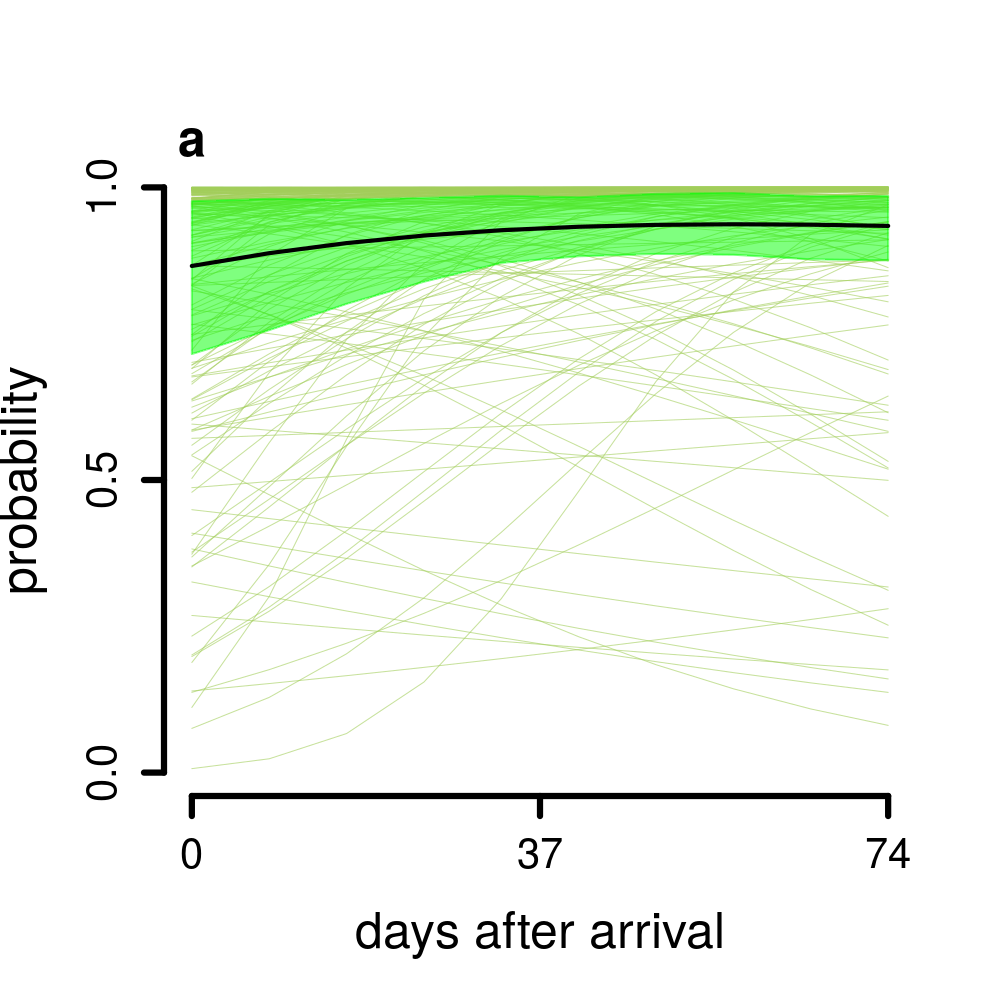
\includegraphics[scale=0.6]{figure_1_a.png}
  \end{subfigure}%
  ~
  \begin{subfigure}{0.5\textwidth}
    \centering
    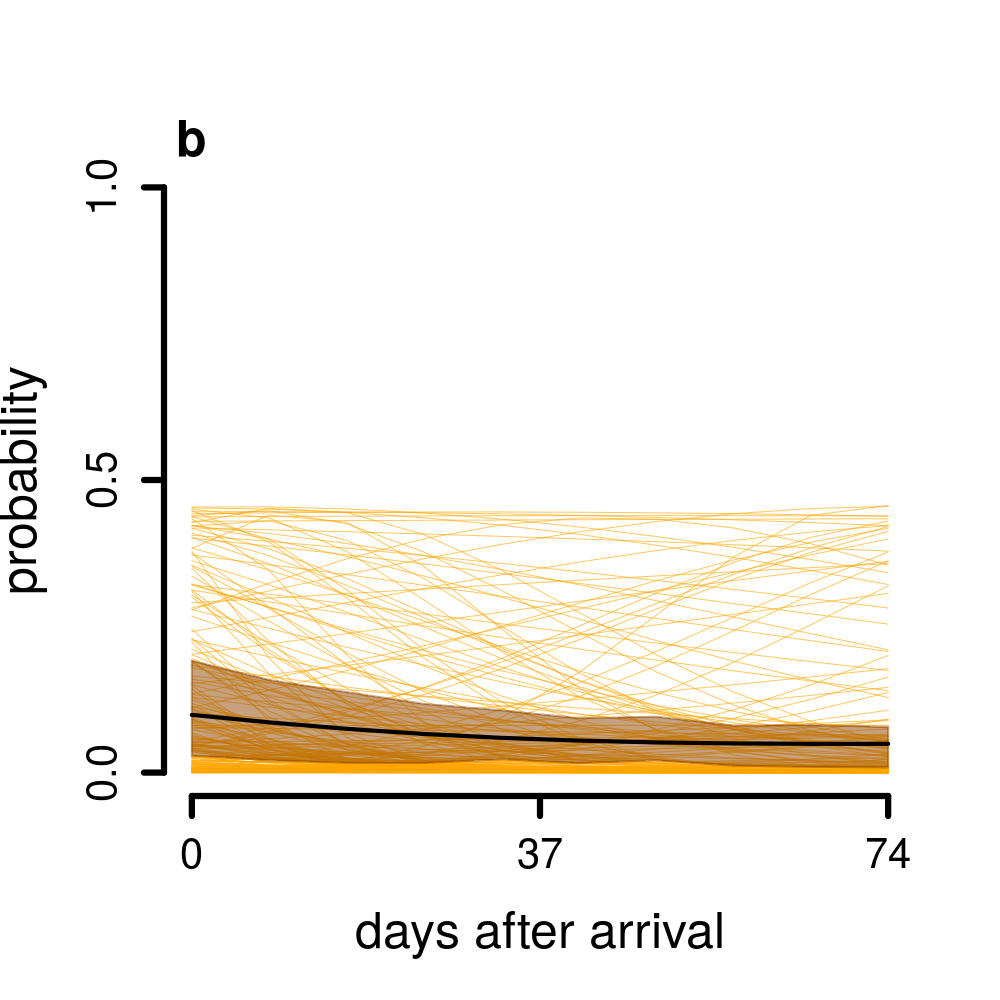
\includegraphics[scale=0.6]{figure_1_b.png}
  \end{subfigure}
  %
  \begin{subfigure}{0.5\textwidth}
    \centering
    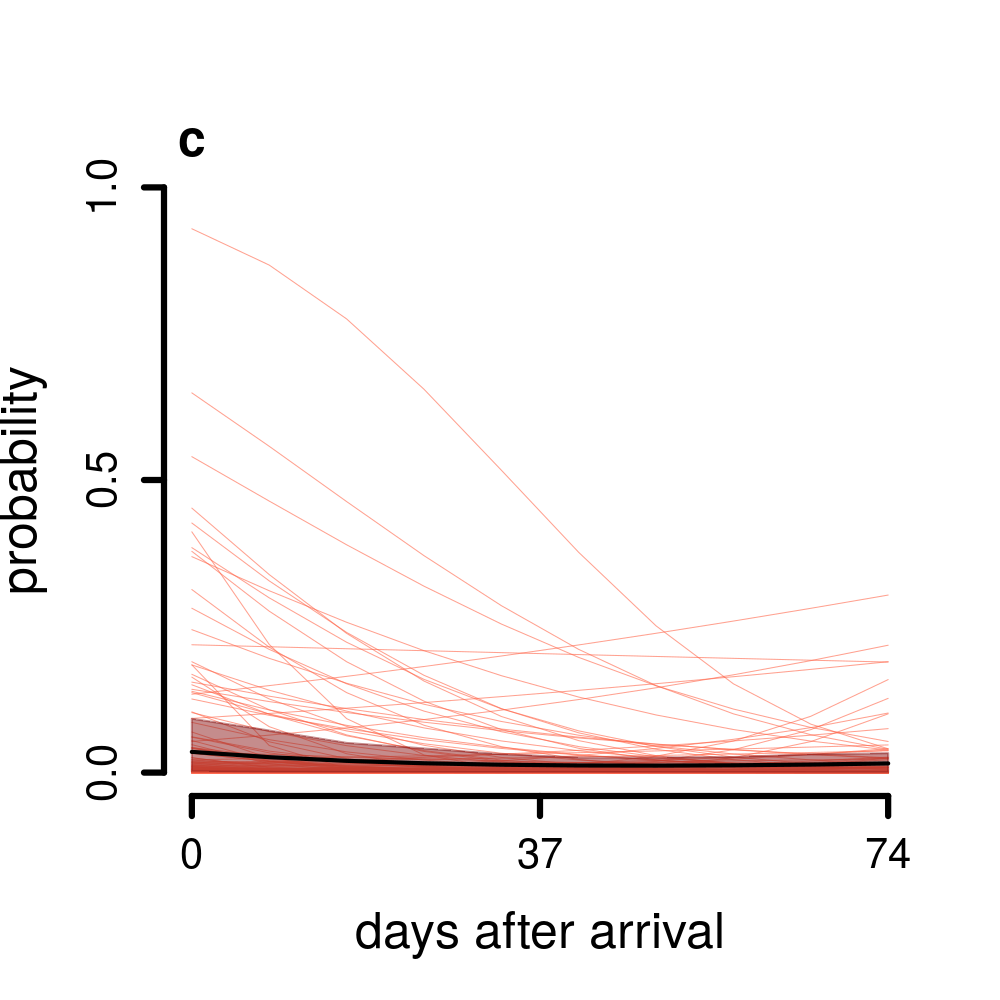
\includegraphics[scale=0.6]{figure_1_c.png}
  \end{subfigure}%
  ~
  \begin{subfigure}{0.5\textwidth}
    \centering
    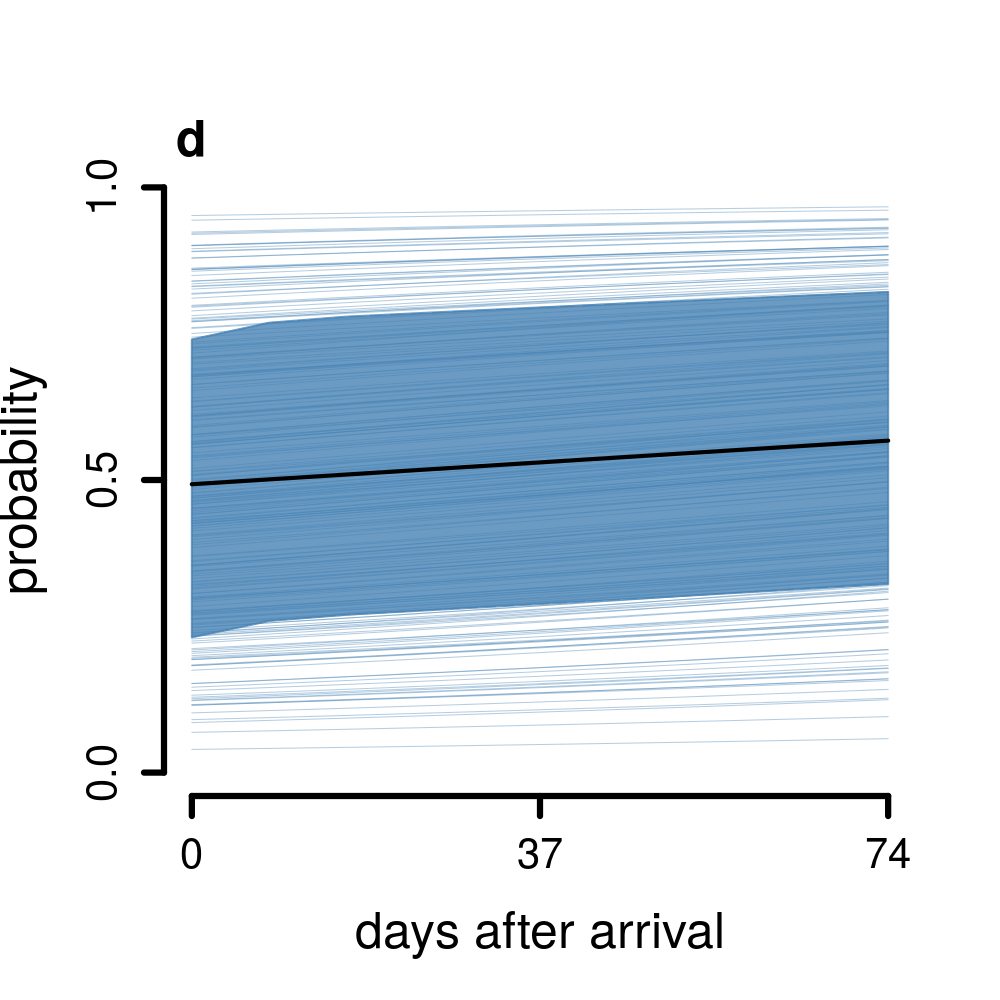
\includegraphics[scale=0.6]{figure_1_d.png}
  \end{subfigure}
  \caption{Probability of green ($a$), amber ($b$), red ($c$) and missing ($d$) codes across days after arrival to the shelter (average length of stay + 1 standard deviation) accounting for variation across dogs, contexts and dog $\times$ context behaviour. Thick black lines show posterior mean estimates, coloured bands show the 95\% highest density interval of the mean, and thin coloured lines ($n = 241$) show one random sample from one randomly-chosen context from each dog's posterior distribution.}
  \label{fig_shelter_behaviour}
\end{figure}

\begin{figure}
  \centering
  \begin{subfigure}{0.5\textwidth}
    \centering
    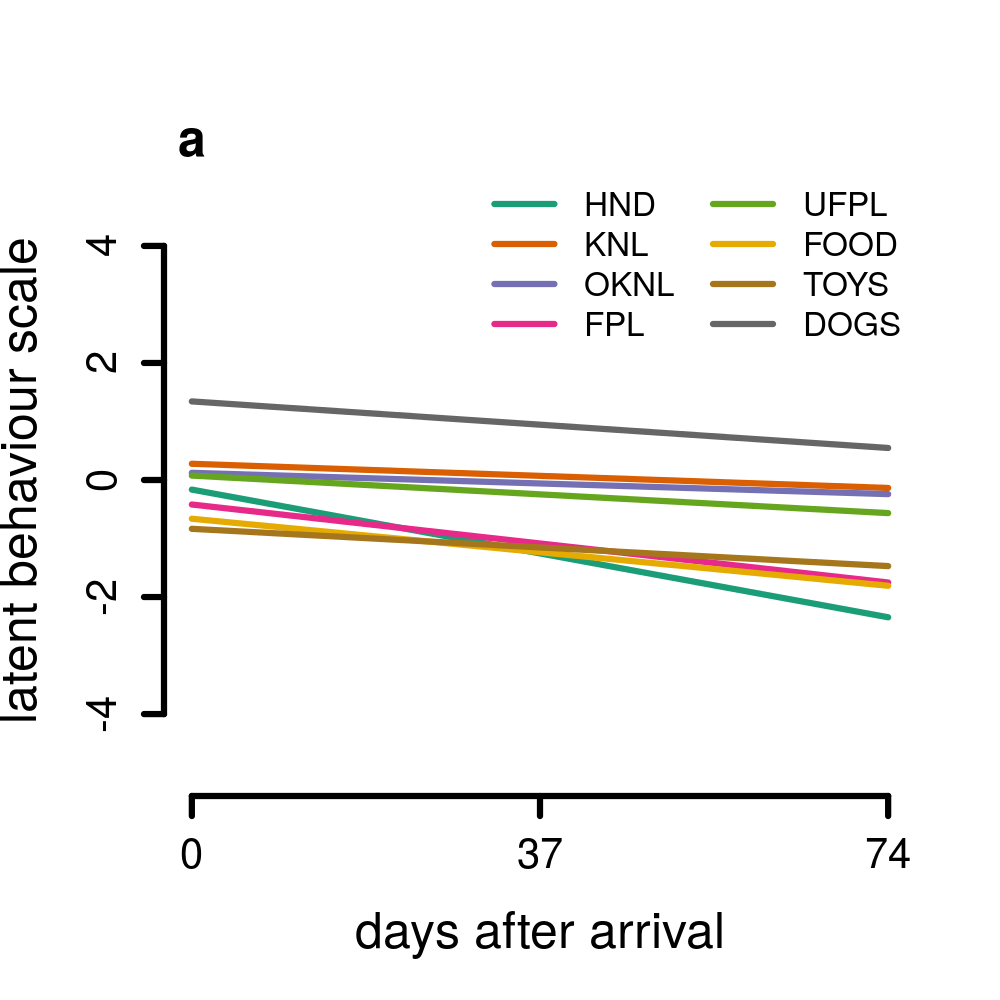
\includegraphics[scale=0.6]{figure_2_a.png}
  \end{subfigure}%
  ~
  \begin{subfigure}{0.5\textwidth}
    \centering
    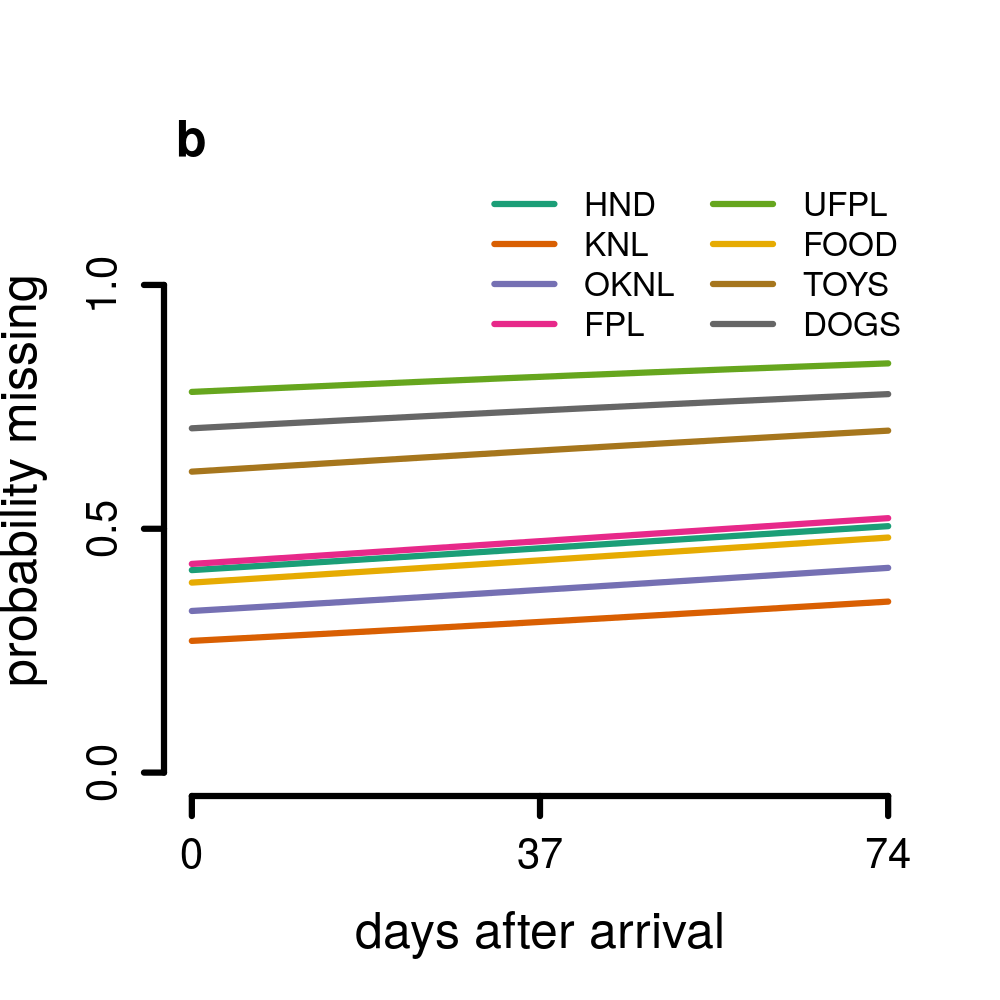
\includegraphics[scale=0.6]{figure_2_b.png}
  \end{subfigure}
  \caption{Variation across contexts for the latent behaviour scale (a) and for the probability of missing data (b) across days after arrival (average length of stay + 1 standard deviation). Lines show posterior mean estimates. Exact estimates with uncertainty provided in Supplementary Material Table S1 and Figures S1a-b.}
\end{figure}

\begin{figure}
  \centering
  \begin{subfigure}{0.5\textwidth}
    \centering
    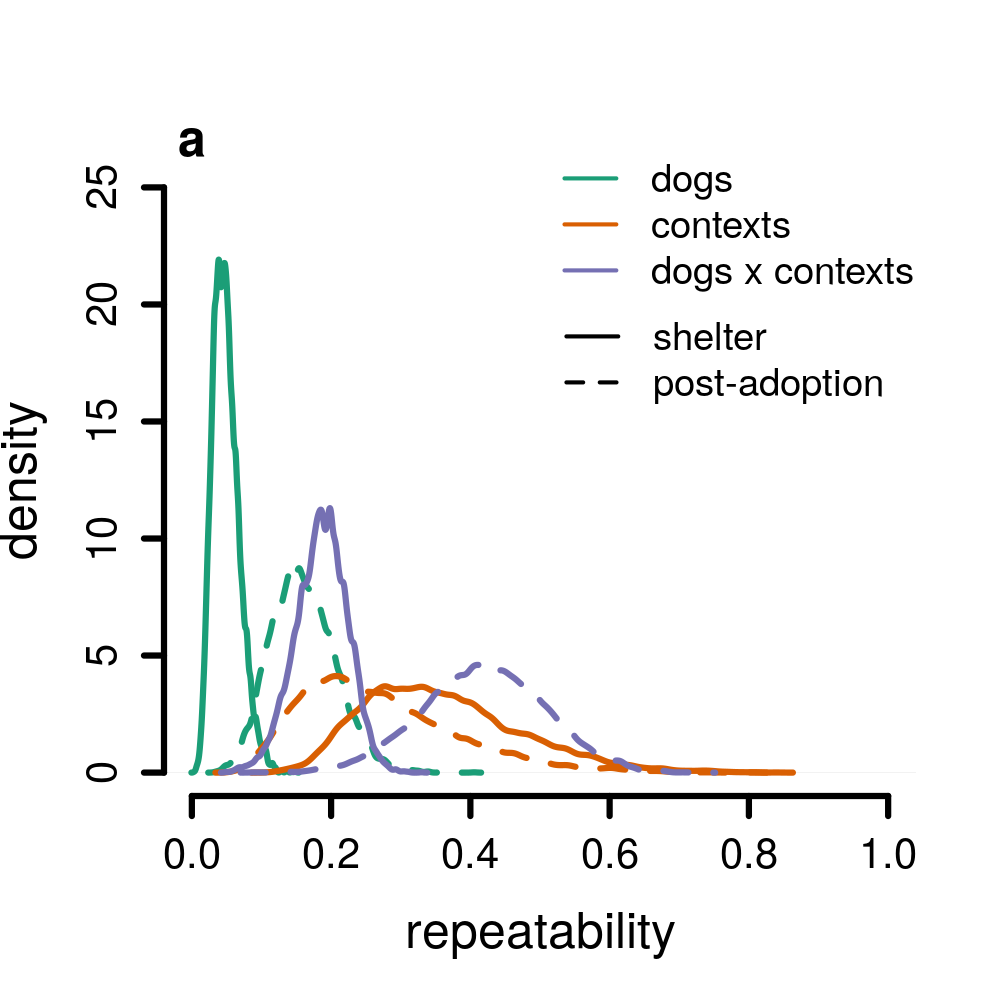
\includegraphics[scale=0.6]{figure_3_a.png}
  \end{subfigure}%
  ~
  \begin{subfigure}{0.5\textwidth}
    \centering
    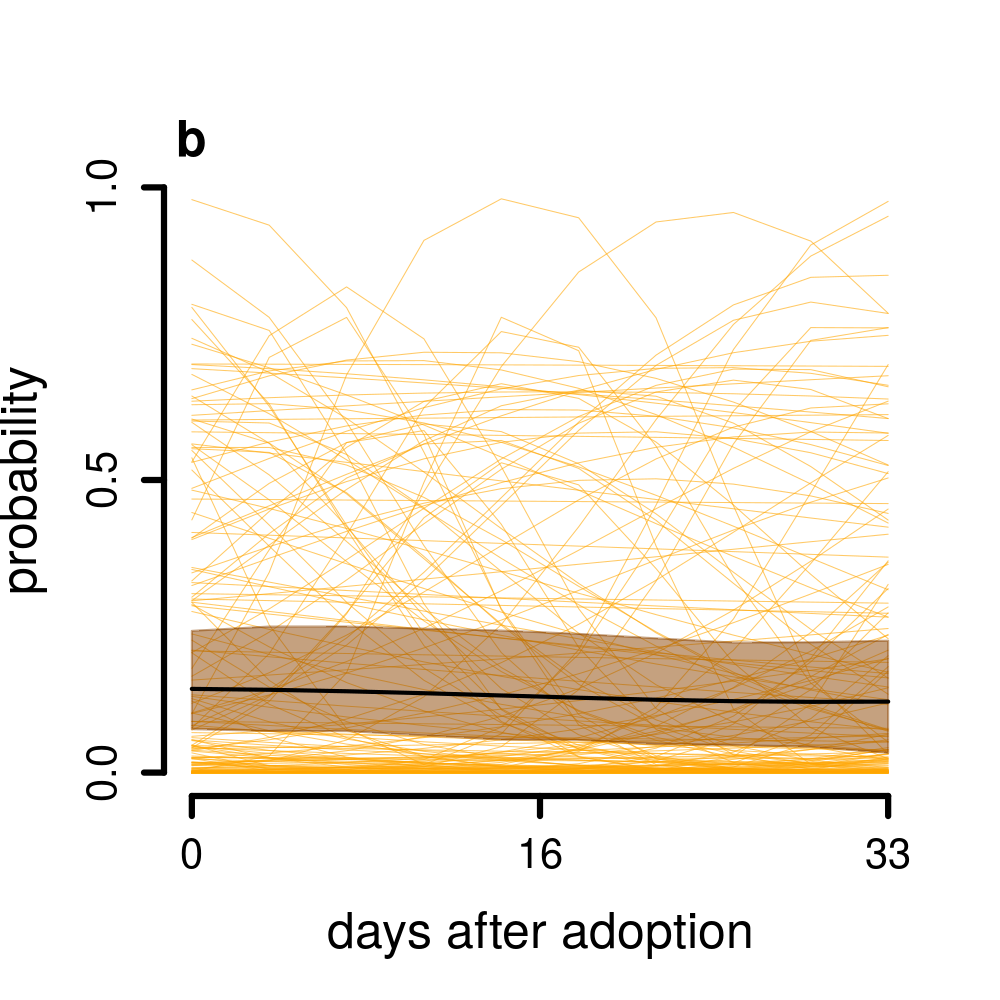
\includegraphics[scale=0.6]{figure_3_b.png}
  \end{subfigure}
  %
  \begin{subfigure}{0.5\textwidth}
    \centering
    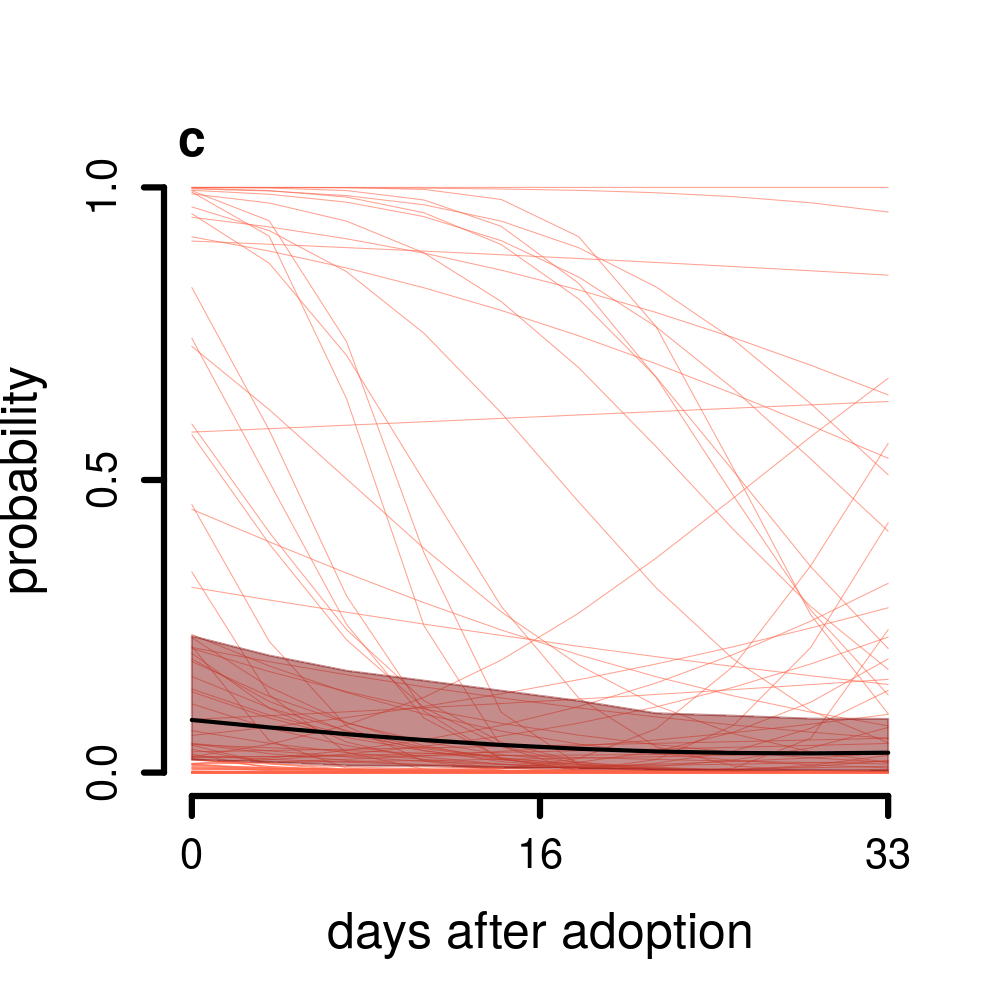
\includegraphics[scale=0.6]{figure_3_c.png}
  \end{subfigure}%
  ~
  \begin{subfigure}{0.5\textwidth}
    \centering
    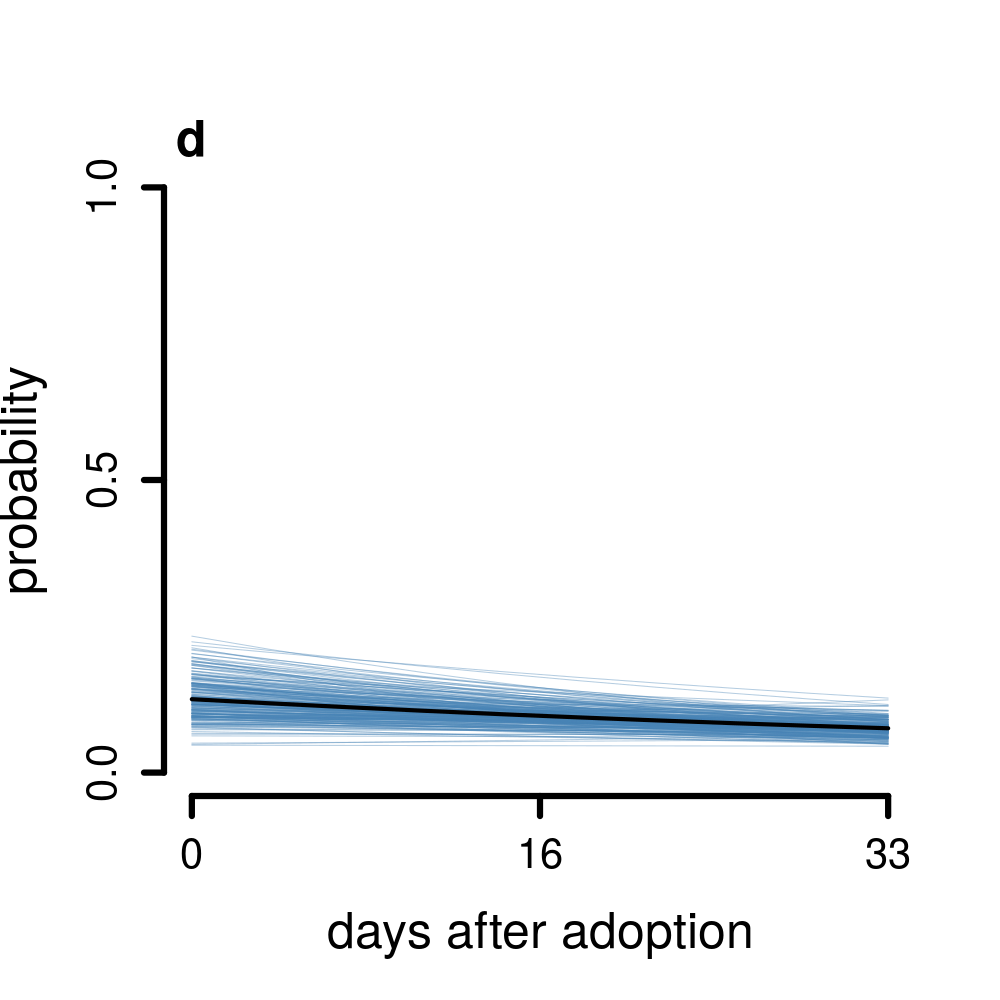
\includegraphics[scale=0.6]{figure_3_d.png}
  \end{subfigure}
  \caption{Probability of green ($a$), amber ($b$), red ($c$) and missing ($d$) codes across days after adoption (average days after adoption interview + 1 standard deviation)  accounting for variation across dogs, contexts and dog $\times$ context behaviour. Thick black lines show posterior mean estimates, coloured bands show the 95\% highest density interval of the mean, and thin coloured lines ($n = 241$) show one random sample from one randomly-chosen context from each dog's posterior distribution.}
  \label{fig_adoption_behaviour}
\end{figure}

\begin{figure}[t!]
  \centering
  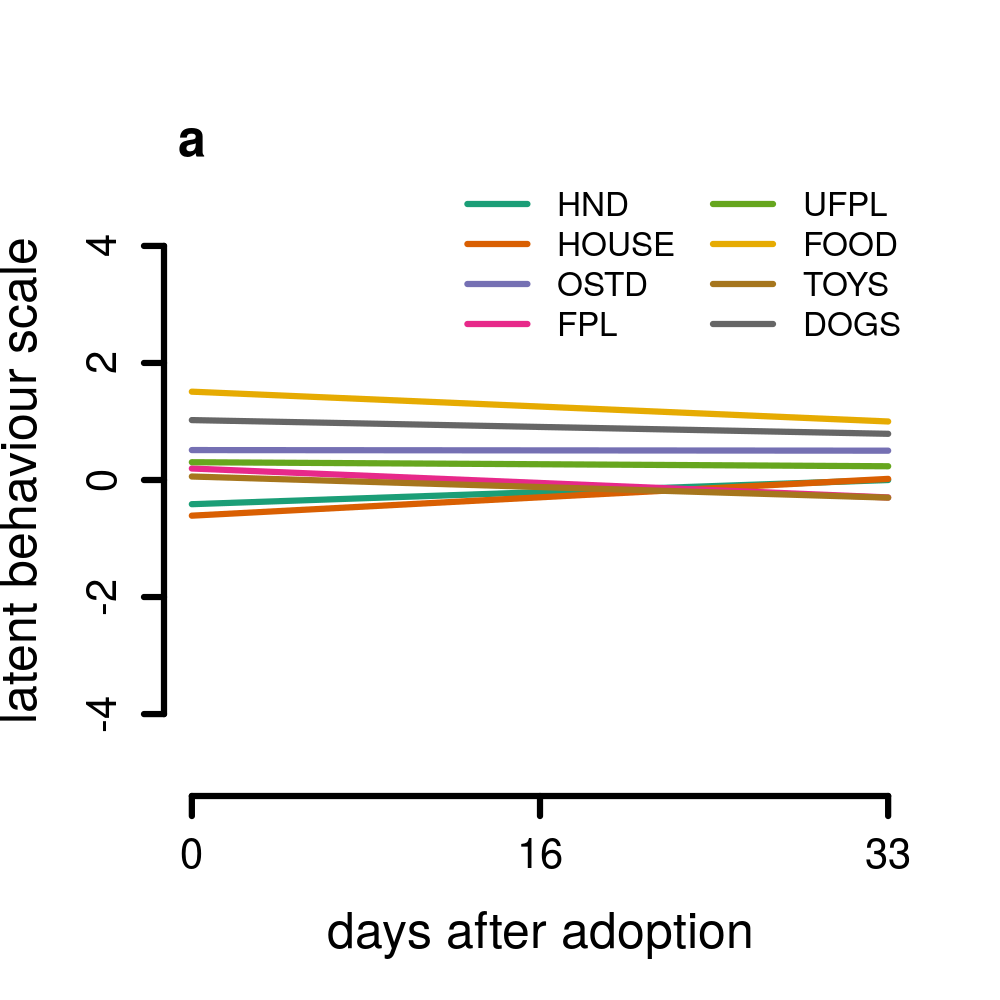
\includegraphics[scale=0.8]{figure_4.png}
  \caption{Variation across contexts for the latent behaviour scale across days after adoption (average days after adoption interview + 1 standard deviation). Lines show posterior mean estimates. Exact estimates with uncertainty provided in Supplementary Material Table S2 and Figures S2.}
\end{figure}

\begin{figure}
  \centering
  \begin{subfigure}{0.5\textwidth}
    \centering
    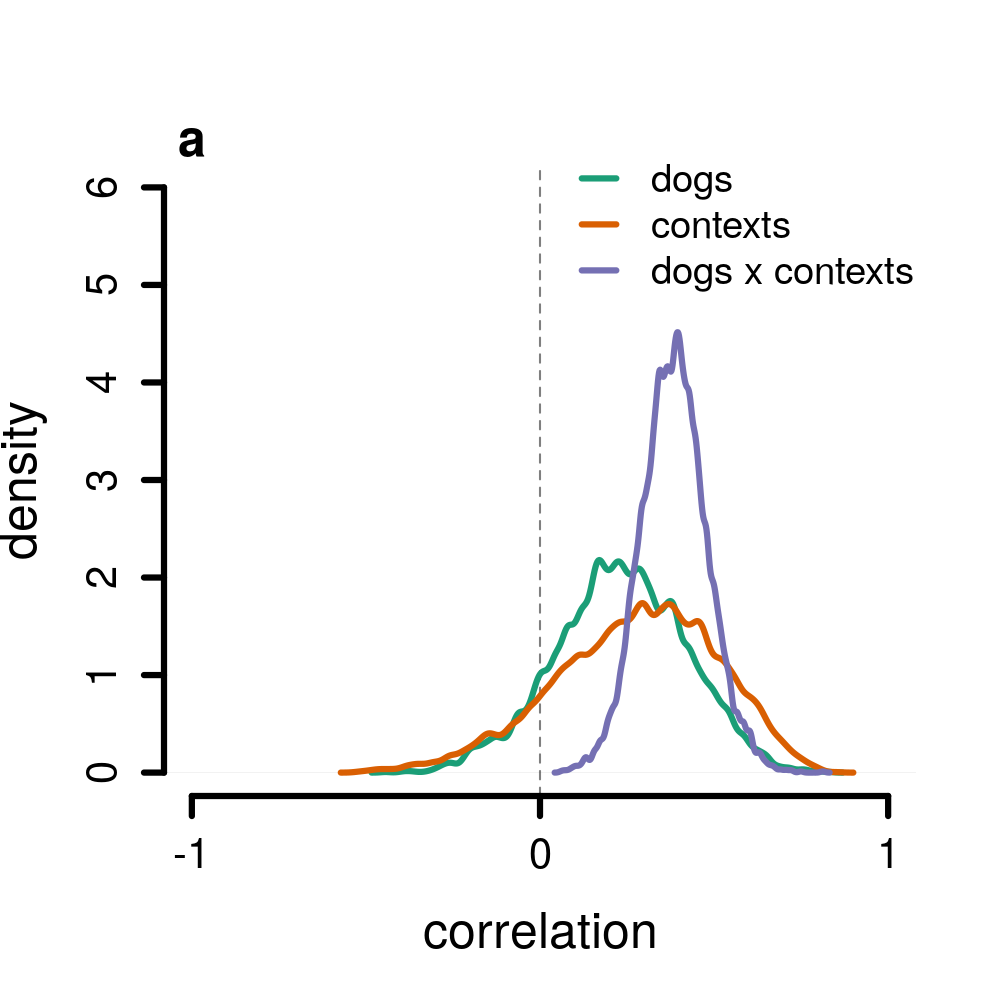
\includegraphics[scale=0.7]{figure_5_a.png}
  \end{subfigure}%
  ~
  \begin{subfigure}{0.5\textwidth}
    \centering
    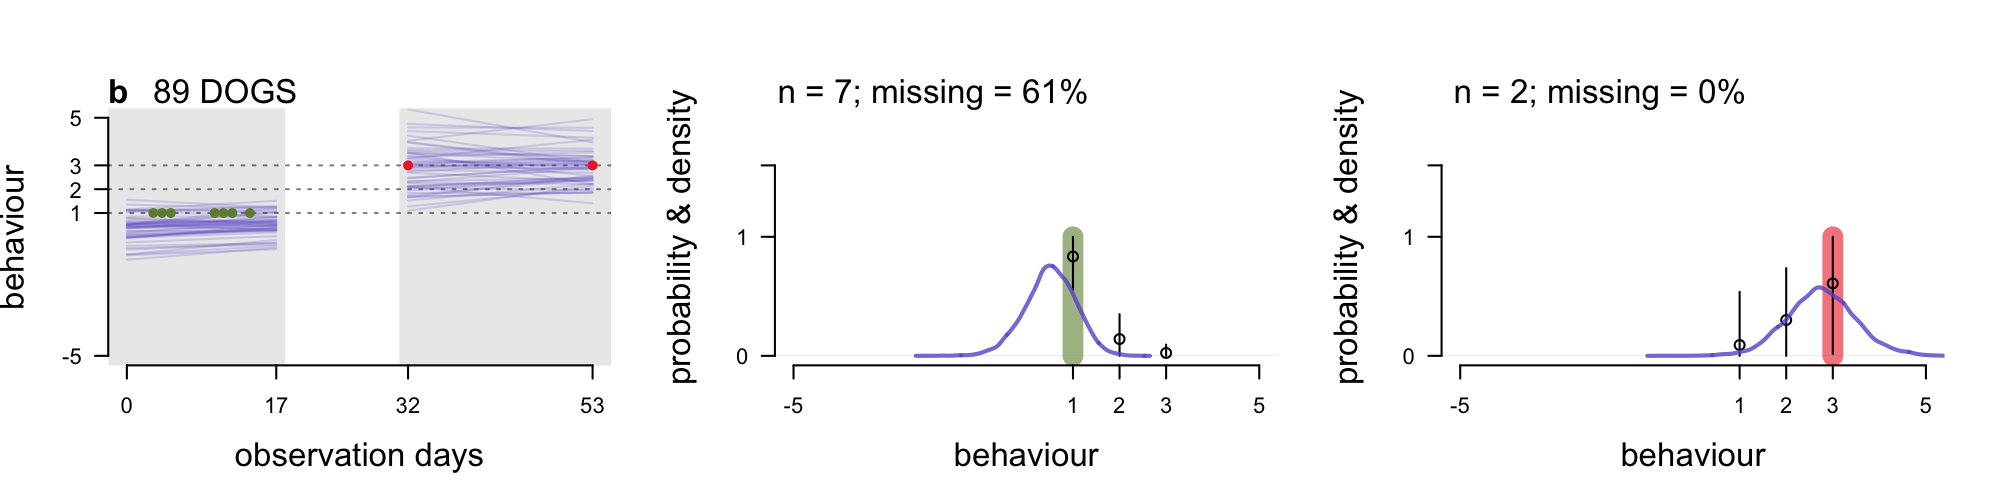
\includegraphics[scale=0.7]{figure_5_b.png}
  \end{subfigure}
  \caption{Correlations (posterior densities) between dog-, context- and dog $\times$ context-varying intercept (personality; a) and slope (plasticity; b) parameters between behaviour recorded at the shelter and behaviour recorded from the post-adoption interviews. Vertical dashed line shows the zero point.}
\end{figure}

\newpage
\printbibliography
\end{document}
